\documentclass[12pt]{article}
\usepackage{bigints}
\usepackage{graphicx}			% Use this package to include images
\usepackage{amsmath}	
\usepackage{amssymb}
\usepackage{amsfonts}
\usepackage{polynom}
% A library of many standard math expressions
\graphicspath{ {./Images/} }
\usepackage[margin=1in]{geometry}% Sets 1in margins. 
\newcommand{\qed}[0]{$\blacksquare$}
\usepackage{fancyhdr}			% Creates headers and footers
\usepackage{enumerate}          %These two package give custom labels to a list
\usepackage[shortlabels]{enumitem}


% Creates the header and footer. You can adjust the look and feel of these here.
\pagestyle{fancy}
\fancyhead[l]{Aditya Gupta}
\fancyhead[c]{Math 134 Homework \#7}
\fancyhead[r]{\today}
\fancyfoot[c]{\thepage}
\renewcommand{\headrulewidth}{0.2pt} %Creates a horizontal line underneath the header
\setlength{\headheight}{15pt} %Sets enough space for the header



\begin{document} 
\begin{enumerate}[start=1,label={\bfseries. },leftmargin=1in]
\item [30. ]The area of the triangle is \( A = \frac{1}{2} \times b \times h = \frac{bh}{2} \), and the centroid \( G = \left( \frac{a+b}{3}, \frac{h}{3} \right) \). The centroid was calculated using the formula $\left(\frac{x_1 + x_2 + x_3}{3},\frac{y_1 + y_2 + y_3}{3}\right)$ 

For the \(y\)-axis: the centroid’s distance \( d_y = \frac{a+b}{3} \), so 
\[
V_y = 2 \pi A d_y = 2 \pi \cdot \frac{bh}{2} \cdot \frac{a+b}{3} = \frac{\pi bh (a+b)}{3}.
\]

For the \(x\)-axis: the centroid’s distance \( d_x = \frac{h}{3} \), so 
\[
V_x = 2 \pi A d_x = 2 \pi \cdot \frac{bh}{2} \cdot \frac{h}{3} = \frac{\pi bh^2}{3}.
\]

Thus, the volumes of revolution are \( V_y = \frac{\pi bh (a+b)}{3} \) and \( V_x = \frac{\pi bh^2}{3} \).

\item [1.]
The following image shows how the proposition is proven. 

    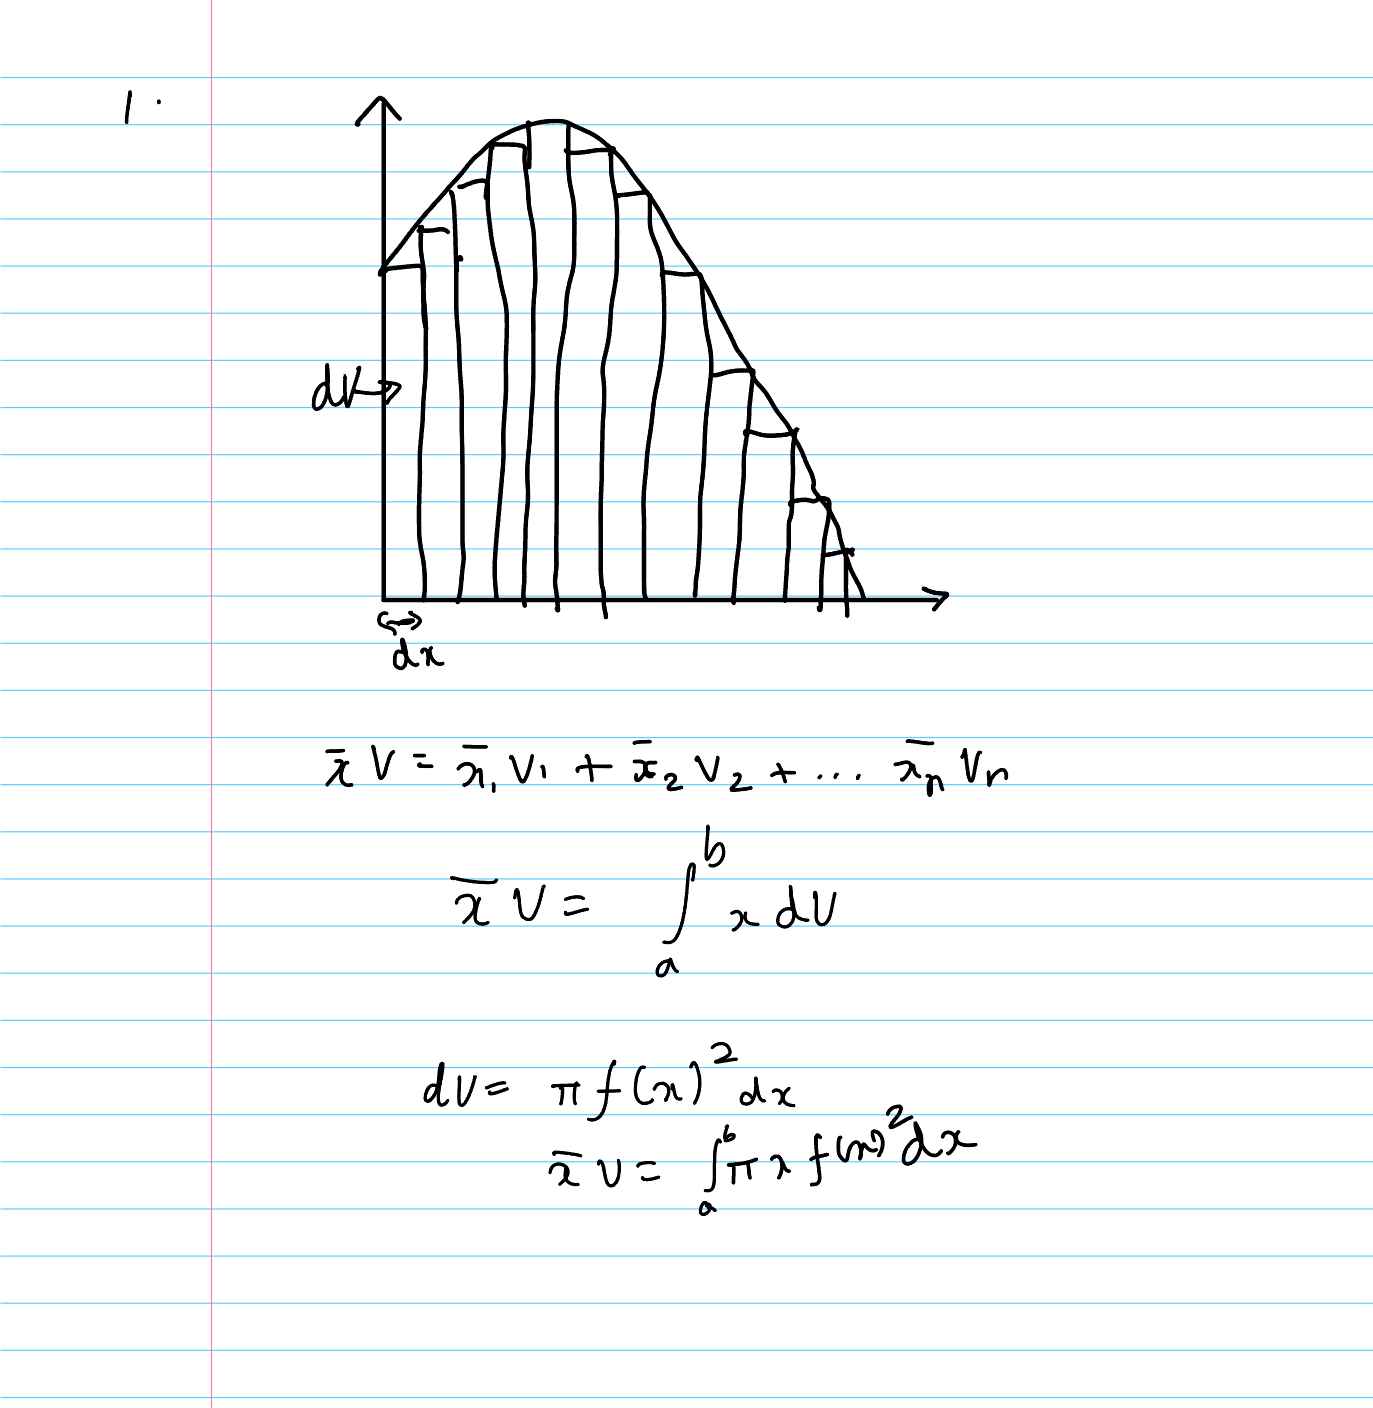
\includegraphics[width=0.75\linewidth]{Math 134//Images/Hw 7.jpeg}
\item [2. ]
The following image shows how the $\bar{y}$ is calculated. Each disc of volume $dV$is rotated around the y axis and

    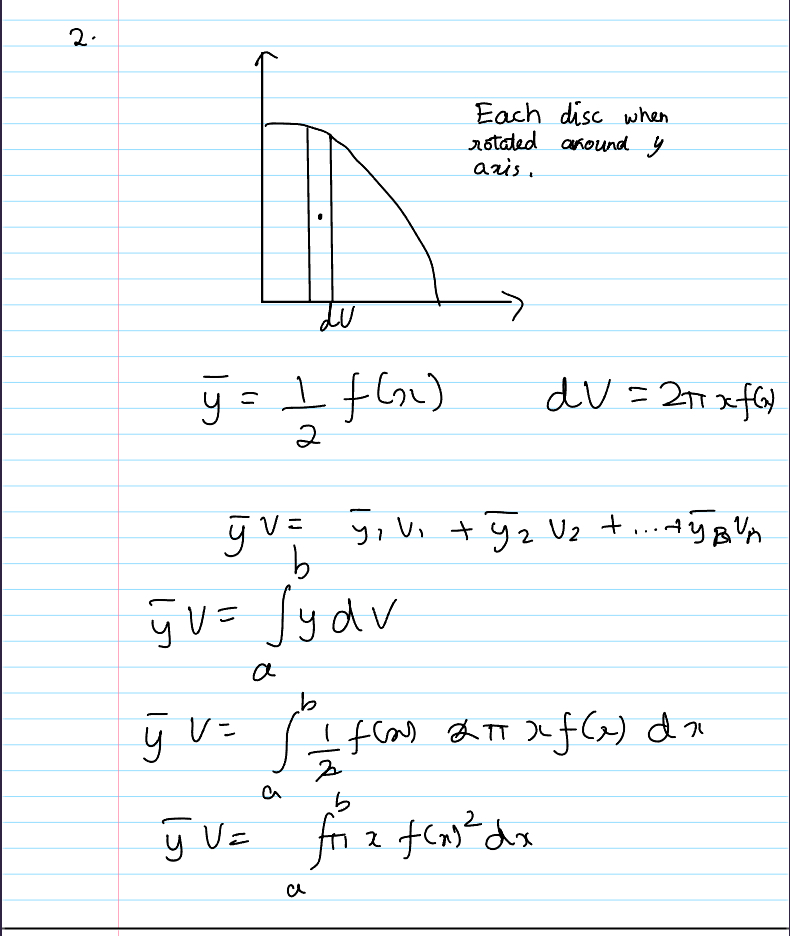
\includegraphics[width=0.75\linewidth]{Math 134//Images/Hw 8.jpeg}

\item [3.d]
Volume of revolution of region between $y=\sqrt{x}$ and x axis:
\[
V_x = \pi\int_0^1 x dx = \pi\left[\frac{x^{2}}{2}\right]_{0}^1 = 0.5\pi
\]

Volume of revolution of region between $y=\sqrt{x}$ and y axis:
\[
V_y = 2\pi \int_{0}^1 x \sqrt{x} dx = 2\pi\left[\frac{x^{2.5}}{2.5}\right]_0^1 = 0.8 \pi
\]

Since 
\[
\Bar{x}V_x = \int_{0}^1 \pi x [f(x)]^2dx
\]
\[
\Bar{x} = \frac{\int_0^1 \pi x^2 dx}{0.5\pi} = \frac{2}{3}
\]
Thus, for the solid around the x axis, the centroid is $\left(\frac{2}{3},0\right)$


Similarly:
\[
\Bar{y} = \frac{\int_0^1 \pi x^2 dx}{0.8\pi} = \frac{5}{12}
\]
Thus, for the solid around the x axis, the centroid is $\left(0,\frac{5}{12}\right)$
\item [40. ]
Given:
    \begin{itemize}
        \item Oil density, \( \sigma = 60 \, \text{lb/ft}^3 \)
        \item Radius of the tank, \( r = 4 \, \text{ft} \)
        \item Height of the cylindrical part, \( h = 8 \, \text{ft} \)
        \item Total height to pump the oil to, \( H = 12 \, \text{ft} \)
    \end{itemize}

    Work for the Cylinder:
    The cross-sectional area at any height \( x \) in the cylinder is a constant \( A(x) = \pi r^2 = 16 \pi \). The work required to pump the oil from the cylindrical part is:
    \[
    W_{\text{cylinder}} = \int_0^8 \sigma x \cdot A(x) \, dx = \int_0^8 60 \cdot x \cdot 16 \pi \, dx = 960 \pi \int_0^8 x \, dx
    \]
    \[
    W_{\text{cylinder}} = 960 \pi \left[ \frac{x^2}{2} \right]_0^8 = 960 \pi \cdot \frac{64}{2} = 30720 \pi \approx 96,510 \, \text{foot-pounds}
    \]

    In the hemisphere part, the cross-sectional area varies with \( x \) and is given by:
    \[
    A(x) = \pi \left( r^2 - (x - 8)^2 \right) = \pi \left( 16 - (x - 8)^2 \right)
    \]
    The work required to pump the oil from this part is:
    \[
    W_{\text{hemisphere}} = \int_8^{12} \sigma x \cdot A(x) \, dx = \int_8^{12} 60 \cdot x \cdot \pi (16 - (x - 8)^2) \, dx
    \]
    \[
    W_{\text{hemisphere}} = 60 \pi \int_8^{12} x (16 - (x - 8)^2) \, dx = 76404 \text{ foot-pounds}
    \]
    Thus total work is:
    \[
    W = W_{\text{cylinder}} + W_{\text{hemisphere}} \approx 96,510 + 76,404 = 172,913 \, \text{foot-pounds}
    \]

    Since $ P = 0.5 hP = 0.5 \cdot 550 = 275 \frac{\text{ft lbs}}{s}$.
    
    Thus total time = $\frac{172913}{275} \approx 629s$

\item [WS3]

Let \( y \) be the height of a thin horizontal slice within the tank. The width of the tank at height \( y \) is given by \( 2 \sqrt{9 - y^2} \), where the radius of the tank is 3. Thus, the volume of the slice is
\[
dV = 12 \times 2 \sqrt{9 - y^2} \, \Delta y.
\]
The weight of the slice is then
\[
\text{Weight} = 750 \times g \times 12 \times 2 \sqrt{9 - y^2} \, \Delta y.
\]

The distance that each slice must be lifted to reach a height of 6.2 meters is \( (6.2 - y) \). Thus, the work done to lift this slice is
\[
dW = 750 \times g \times 12 \times 2 \sqrt{9 - y^2} (6.2 - y) \, dy.
\]
The total work done in pumping all the gasoline is then
\[
\text{Work} = \int_{-3}^0 750 \times g \times 12 \times 2 \sqrt{9 - y^2} (6.2 - y) \, dy.
\]

Simplifying, we get
\[
\text{Work} = 18000 g \left( 6.2 \int_{-3}^0 \sqrt{9 - y^2} \, dy - \int_{-3}^0 y \sqrt{9 - y^2} \, dy \right).
\]
The integral \( \int_{-3}^0 \sqrt{9 - y^2} \, dy \) represents the area of a semicircle with radius 3, which equals \( \frac{9\pi}{2} \). The second integral can be evaluated as
\[
\int_{-3}^0 y \sqrt{9 - y^2} \, dy = \frac{1}{3} (9 - y^2)^{3/2} \Big|_{-3}^0 = 9.
\]
Substituting, we obtain
\[
\text{Work} = 18000 g \left( 6.2 \cdot \frac{9\pi}{2} + 9 \right).
\]

\textbf{(b)} To confirm this result using the center of mass, we express the work as the weight of the gasoline multiplied by the distance that its center of mass travels.

From part (a), we have
\[
dV = 12 \times 2 \sqrt{9 - y^2} \, dy.
\]
The volume, mass, and weight of the gasoline are given by
\[
\text{Volume} = \int_{-3}^0 dV, \quad \text{Mass} = \rho \int_{-3}^0 dV, \quad \text{Weight} = g \rho \int_{-3}^0 dV.
\]
The moment is
\[
\text{Moment} = \rho \int_{-3}^0 y \, dV,
\]
and the work is
\[
\text{Work} = g \rho \int_{-3}^0 (6.2 - y) \, dV.
\]

The work can also be written as
\[
\text{Work} = \text{Weight} \times (6.2 - \bar{y}),
\]
where \( \bar{y} \) is the \( y \)-coordinate of the center of mass, calculated as
\[
\bar{y} = \frac{\int_{-3}^0 y \, dV}{\int_{-3}^0 dV}.
\]
Therefore,
\[
\text{Work} = g \rho \int_{-3}^0 dV \times \left( 6.2 - \frac{\rho \int_{-3}^0 y \, dV}{\rho \int_{-3}^0 dV} \right).
\]
Expanding and simplifying, we confirm that this expression is equivalent to the integral we set up in part (a), thereby verifying that the work done equals the weight of the gasoline times the distance the center of mass travels.

\item [52. ]

Using the Fundamental Theorem of Calculus, we differentiate $f(x)$:

\[
f'(x) = \frac{d}{dx} \left( \int_1^{2x} \sqrt{16 + t^4} \, dt \right)
\]

By the chain rule:

\[
f'(x) = 2 \cdot \sqrt{16 + (2x)^4}
\]

This simplifies to:

\[
f'(x) = 2 \sqrt{16 + 16x^4}
\]

Since $16 + 16x^4 > 0$ for all $x$, it follows that:

\[
f'(x) > 0
\]

Thus, $f(x)$ is strictly increasing for all $x > 0$, meaning that $f(x)$ is one-to-one and therefore has an inverse.

To find $(f^{-1})'(0)$, we use the formula for the derivative of the inverse function:

\[
(f^{-1})'(y) = \frac{1}{f'(f^{-1}(y))}
\]

We need to find $x_0 = f^{-1}(0)$, which means solving for $x_0$ such that:

\[
f(x_0) = 0
\]

From the definition of $f(x) = \int_1^{2x} \sqrt{16 + t^4} dt$, we set this equal to zero:

\[
\int_1^{2x_0} \sqrt{16 + t^4} dt = 0
\]

The only way this integral can be zero is if the limits of integration are equal, meaning:

\[
2x_0 = 1
\]

Thus, $x_0 = \frac{1}{2}$ and therefore $f^{-1}(0) = \frac{1}{2}$.

Next, we compute $(f^{-1})'(0) = \frac{1}{f'(\frac{1}{2})}$. Using the expression for $f'(x) = 2\sqrt{16 + 16x^4}$, we substitute $x = \frac{1}{2}$:

\[
f'\left( \frac{1}{2} \right) = 2\sqrt{16 + 16\left(\frac{1}{2}\right)^4} = 2\sqrt{16 + 1} = 2\sqrt{17}
\]

Thus:

\[
(f^{-1})'(0) = \frac{1}{2\sqrt{17}}
\]

\item [66. ]
\[
\frac{d^n}{dx^n}\left(\ln(1-x)\right) = (-1)^n(n-1)!(x-1)^{-n}
\]

 \item [72. ]
 Given:
 \[
 x>0
 \]
 \[
 x > \ln(1)
 \]
 Thus, we may say that:
 \[
 x  > \ln(1)\times \ln(x) \times\ln\left(\frac{x^2}{2!}\right)\times\ln\left(\frac{x^3}{3!}\right)
 \times ... \times  \ln\left(\frac{x^n}{n!}\right)\] 

as the RHS is still 0.

Raising each side as power of e and using the additive property of ln functions:
\[
e^x > e^{ln\left( 1 + x + \frac{x^2}{2!} + \frac{x^3}{3!} + ... +\frac{x^n}{n!}\right)}
\]

Simplifying the RHS:
\[
e^x > \left( 1 + x + \frac{x^2}{2!} + \frac{x^3}{3!} + ... +\frac{x^n}{n!}\right)
\blacksquare
\]

\item [73. ]Following from previous question:

\[
e^x >  1 + x + \frac{x^2}{2!} + \frac{x^3}{3!} + ... +\frac{x^{n+1}}{(n+1)!} > \frac{x^{n+1}}{(n+1)!}
\]
To prove this for a sufficiently large x:
\[
\frac{x^{n+1}}{(n+1)!} > x^n
\]

We may choose an $x > (n+1)!$

So:
\[
\frac{x^{n+1}}{x^n} > (n+1)!
\]
Rearranging terms:
\[
\frac{x^{n+1}}{(n+1)!} > x^n
\]


Thus, we may say that for a sufficiently large x, the proposition holds.
\item [70.] Let \( x \) be the distance of the person along the path from the point closest to the spotlight, and let \( \theta \) be the angle of the spotlight from the perpendicular line to the path.

Given \( \frac{dx}{dt} = 6 \) feet/second, the spotlight is 30 feet from the path, and \( x = 50 \) feet at the moment of interest. We have: 
\[
tan (\theta) = \frac{x}{30} 
\]
Differentiating with respect to \( t \): 
\[
\sec^2 \theta \cdot \frac{d\theta}{dt} = \frac{1}{30} \cdot \frac{dx}{dt} \Rightarrow \frac{d\theta}{dt} = \frac{\frac{1}{30} \cdot \frac{dx}{dt}}{\sec^2 \theta}
\]
Substitute \( \tan \theta = \frac{50}{30} = \frac{5}{3} \), and use \( \sec^2 \theta = 1 + \tan^2 \theta = \frac{34}{9} \). Then:
\[
\frac{d\theta}{dt} = \frac{\frac{1}{30} \cdot 6}{\frac{34}{9}} = \frac{1}{5} \cdot \frac{9}{34} = \frac{9}{170}
\]
Thus, the spotlight is turning at \( \frac{9}{170} \) radians per second.

\end{enumerate} 
\end{document}
